\begin{pa} \label{PA:9.8} In earlier investigations, we have used
  integration to calculate quantities such as area, volume, mass, and
  work.  We are now interested in determining the 
  length of a space curve.

  Consider the smooth curve in 3-space defined by the vector-valued
  function
    \[\vr(t) = \langle x(t), y(t), z(t) \rangle = \langle \cos(t), \sin(t), t \rangle\]
    for $t$ in the interval $[0,2\pi]$. A picture of the graph of $\vr$ is shown in Figure \ref{F:9.8.Arc_length_3d}.
\begin{figure}[ht]
\begin{center}
\begin{minipage}{2.5in}
\begin{center}
%\resizebox{!}{2.25in}{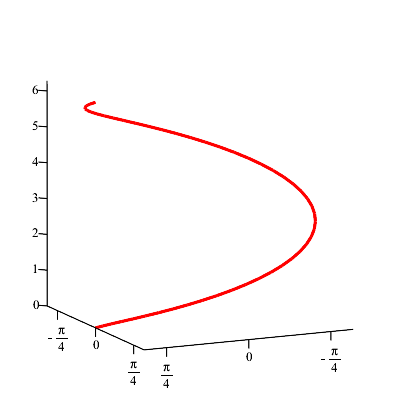
\includegraphics[trim=0cm 0.0cm 0.25cm 1.5cm, clip]{9_8_Arc_length_3D}}
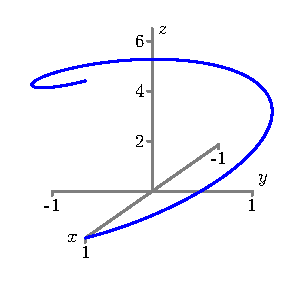
\includegraphics{figures/fig_9_8_length_1.eps}
\end{center}
\caption{The graph of $\vr$.}
\label{F:9.8.Arc_length_3d}
\end{minipage} \hspace{0.5in}
\begin{minipage}{2.5in}
\begin{center}
%\resizebox{!}{2.25in}{\animategraphics[controls,trim=0cm 0.0cm 0.25cm 1.5cm]{4}{9_8_AL3D_}{01}{20}}
\animategraphics[controls]{2}{figures/fig_9_8_length_animate_}{00}{24}
\end{center}
\caption{Approximating the length of the curve.}
\label{F:9.8.Arc_length_3d_animation}
\end{minipage}
\end{center}
\end{figure}
%crop graphics in animate trim=<left> <bottom> <right> <top>, add, clip with \includegraphics
%Write the coordinates of the points on the curve determined by the endpoints of the interval $[x_{i-1},x_i]$.
    \ba
    \item The animation in Figure \ref{F:9.8.Arc_length_3d_animation} illustrates the process of approximating the length of the curve defined by $\vr(t)$ on the interval $[0,2\pi]$. Run the animation and explain what is happening.

\begin{comment}

We are partitioning the interval $[a,b]$ into $n$ subintervals of equal length and approximating the length of the curve on each subinterval by the length of the segment connecting the endpoints. We then add these approximations on the subintervals together to obtain an approximation of the length of the curve.

\as

\end{comment}

    \item Partition the interval $[0,2\pi]$ into $n$ subintervals of equal length and let $0 = t_0 < t_1 < t_2 < \cdots < tn = b$ be the endpoints of the subintervals. Write a formula to approximate the length of the curve on the $i$th subinterval $[t_{i-1},t_i]$. (Hint: the animation in Figure \ref{F:9.8.Arc_length_3d_animation} implies that you should use the length of an appropriate line segment.)

\begin{comment}

The length of the line segment connecting the points $\vr(t_{i-1})$ and $\vr(t_i)$ is given by the distance formula
\[\sqrt{(x_i-x_{i-1})^2+(y_{i}-y_{i-1})^2 + (z_{i}-z_{i-1})^2}.\]

\as

\end{comment}

    \item Use your formula in part (b) to write a sum that adds all of the approximations to the lengths on each subinterval.

\begin{comment}

We add the lengths given in part (b) to obtain the sum
\[\sum_{i=1}^n \sqrt{(x_i-x_{i-1})^2+(y_{i}-y_{i-1})^2 + (z_{i}-z_{i-1})^2}\]
that approximates the total length of the graph of $\vr(t)$ on the interval $[0,2 \pi]$.

\as

\end{comment}

    \item What do we need to do with the sum in part (c) in order to obtain the exact value of the length of the graph of $\vr(t)$ on the interval $[0,2\pi]$?

\begin{comment}

We must take the limit of the sum as $n$ goes to infinity.

\as

\end{comment}

    \ea


\end{pa} \afterpa 